
\documentclass[usenames,dvipsnames]{beamer}
\mode<presentation>{\usetheme{Warsaw}}
\usepackage{textpos} %package for text positioning

%%%%%%%%%%%%%%%%%%%%%%%%%%%%%%%%%%%%%%%%%%%%%%%%%%%%%%%%%%%%%%%%%%%%%%%%%%%%%%%%%%%%
%Normal Math Packages
\usepackage{amsmath}
\usepackage{amsfonts}
\usepackage{enumerate}
\usepackage{amsmath}
\usepackage{mathtools}
\usepackage{tikz-cd}
\usepackage{ragged2e}
\usepackage{mathrsfs}
%%%%%%%%%%%%%%%%%%%%%%%%%%%%%%%%%%%%%%%%%%%%%%%%%%%%%%%%%%%%%%%%%%%%%%%%%%%%%%%%%%%%

%%%%%%%%%%%%%%%%%%%%%%%%%%%%%%%%%%%%%%%%%%%%%%%%%%%%%%%%%%%%%%%%%%%%%%%%%%%%%%%%%%%%
%Created Commands
\theoremstyle{definition}
\newtheorem*{remark}{Remark}
\newtheorem*{question}{Question}
%\newtheorem*{definition}{Definition}
%\newtheorem*{definitions}{Definitions}

\theoremstyle{theorem}
\newtheorem*{proposition}{Proposition}
\newtheorem*{axiom}{Axiom}

\newcommand{\R}{\mathbb{R}}
\newcommand{\Q}{\mathbb{Q}}
\newcommand{\F}{\mathbb{F}}
\newcommand{\A}{\mathcal{A}}
\newcommand{\N}{\mathbb{N}}
\newcommand{\C}{\mathbb{C}}
\newcommand{\opO}{\mathcal{O}}
\newcommand{\states}{\mathcal{S}}
%%%%%%%%%%%%%%%%%%%%%%%%%%%%%%%%%%%%%%%%%%%%%%%%%%%%%%%%%%%%%%%%%%%%%%%%%%%%%%%%%%%%


%%%%%%%%%%%%%%%%%%%%%%%%%%%%%%%%%%%%%%%%%%%%%%%%%%%%%%%%%%%%%%%%%%%%%%%%%%%%%%%%%%%%
%Stuff to make things look good
% Color modification
\setbeamercolor{structure}{fg=green!30!black}% to modify  immediately all palettes
\setbeamercolor{title}{fg=white}
\setbeamercolor{title in head/foot}{fg=yellow}

%Size Modification
\setbeamerfont{frametitle}{size=\small}

% position the logo
\addtobeamertemplate{frametitle}{}{%
\begin{textblock*}{1cm}(\textwidth,-1.1cm)

\includegraphics[height=.9cm,width=.9cm,keepaspectratio]{csu.png}
\end{textblock*}}

% Text Positioning
\usepackage[absolute,overlay]{textpos}
%%%%%%%%%%%%%%%%%%%%%%%%%%%%%%%%%%%%%%%%%%%%%%%%%%%%%%%%%%%%%%%%%%%%%%%%%%%%%%%%%%%%

%Font
%\fontfamily{cmr}\selectfont
\usefonttheme{serif}

%Colors and stuf
\usepackage{color, soul, xcolor} % Colored text and highlighting, respectively
\usepackage{tikz-cd} % For commutative diagrams

%% preamble
\title{Introduction to Riemannian Geometry}
\author{Colin Roberts}

\begin{document}

%%Title Frame
{
\setbeamertemplate{headline}{}
\addtobeamertemplate{frametitle}{\vspace*{-0.9\baselineskip}}{}
\begin{frame}
\titlepage
\end{frame}
}


\AtBeginSection[]
{
	\begin{frame}{Table of Contents}
		\tableofcontents[currentsection]
	\end{frame}
}
%%%%%%%%%%%%%%%%%%%%%%%%%%%%%%%%%%%%%%%%%%%%%%%%%%%%%%%%%%%%%%%%%%%%%%%%%%%%%%%
        \begin{frame}{Motivation and Physical Insight}
            \begin{paragraph}
                \textit{``A unified theory of the physical world calls for a unified mathematical language to help develop and express it."}
            \end{paragraph}
            \vspace*{0.5cm}
            -- Preface of \textbf{Clifford Algebra to Geometric Calculus}, Hestenes \& Sobczyk.
        \end{frame}

        \begin{frame}{Motivation and Physical Insight}
            
            \begin{paragraph}
            Classically, we live in a \emph{metric space} with \emph{no origin}.  Where \emph{measurements} are \emph{real valued} and made \emph{continuously}.  \emph{Coordinates}, \emph{dimensions}, and \emph{units} are imposed by humans and differing choices of these cannot affect measurement.  
            \end{paragraph}
            
            \vspace*{1cm}
            
            \begin{question}
            How do we take each italicized term and turn it into a unified mathematical statement?
            \end{question}
        \end{frame}
        
        \begin{frame}{Motivation and Physical Insight}
            \begin{itemize}
                \item \textbf{Metric space:} Locally looks like $\mathbb{E}^3$ and we can measure distances.
                \item \textbf{No origin:} The space is affine.  It is \textunderline{not} a vector space!
                \item \textbf{Measurements:} Functions on a space. Smoothness depends on the situation. 
                \item \textbf{Continuously:} We can measure quantities at all points in spacetime.
                \item \textbf{Coordinates:} The only way to describe locations in spacetime.
                \item \textbf{Dimensions:} Data and measurement on a space has fundamental physical dimensions.
                \item \textbf{Units:} How we describe dimensions. 
            \end{itemize}
        \end{frame}
        
        \begin{frame}{Measurement and Functions}
            We should only be able to understand the space we live in by measuring it.  There is no knowledge to be had about our universe otherwise.  
            \vspace*{0.5cm}
            
            Said mathematically: we only understand manifolds by functions involving them.
        \end{frame}


\section{Smooth Manifolds}
    
    \subsection{Differential Topology}
        \begin{frame}{Topology}
            \begin{paragraph}
                We need to develop the proper space to do all physical theory in.  We need to satisfy our earlier statement and remove pathologies.
            \end{paragraph}
            \begin{definitions}~
                \begin{enumerate}[(a)]
                    \item A \textbf{topological space} is a ...
                    \item A \textbf{homeomorphism}...
                    \item A topological space is \textbf{Hausdorff} ...
                    \item A topological space is \textbf{locally Euclidean}...
                \end{enumerate}
            \end{definitions}
        \end{frame}
        
        \begin{frame}{Topology}
            \begin{definition}
                A \textbf{topological space} is a set $X$ along with a collection of sets $\{U_\alpha\}_{\alpha \in A}$ that we call open. $X,\emptyset \in \{U_\alpha\}$ and arbitrary unions as well as finite intersections of elements in $\{U_\alpha\}$ are also in $\{U_\alpha\}$.
            \end{definition}
        \end{frame}
        
        \begin{frame}{Topology}
            \begin{definition}
                A \textbf{homeomorphism} is a continuous invertible function $h\colon X \to Y$ with continuous inverse. 
            \end{definition}
            \begin{remark}
                Picturing a topological space as a rubber sheet, homeomorphisms are the ``nice" ways of stretching and bending an object.
            \end{remark}
        \end{frame}
        
        \begin{frame}{Topology}
            \begin{definition}
                A topological space $X$ is \textbf{Hausdorff} if there exists disjoint open neighborhoods for each pair of points $x_1\neq x_2 \in X$.
            \end{definition}
        \end{frame}
        
        \begin{frame}{Topology}
            \begin{definition}
                A topological space $X$ is \textbf{locally Euclidean} if it is a Hausdorff space where each point has a neighborhood homeomorphic to an open subset of Euclidean space $\R^m$.
            \end{definition}
        \end{frame}
        
        \begin{frame}{Topology}
            \begin{paragraph}
                All of this was to build up to a topological manifold.  Which, forgetting jargon, is a space that  (as long as you don't look too far away) looks like the space we live in.
            \end{paragraph}
            \begin{definition}
                A \textbf{topological manifold $M$ of dimension $m$} is a locally Euclidean space.  
            \end{definition}
            \begin{remark}
                Often you will see extra conditions like \emph{paracompact} or \emph{second-countable}, but these are rather unimportant at the moment.
            \end{remark}
        \end{frame}
        
        \begin{frame}{Examples of Topological Manifolds}
            \begin{itemize}
                \item $\R^n$
                \item $\R^n\setminus \{0\}$
                \item $S^n$
                \item $T^n = \underbrace{S^1 \times \cdots \times S^1}_{\textrm{$n$ times}}$
                \item Simplicies
                \item $[0,1]^n$
                \item \st{Cone}
            \end{itemize}
        \end{frame}
        
        \begin{frame}{Smooth Manifold Structure}
            To decide whether a manifold is smooth, we need to understand the functions on it. Most importantly, take the \textbf{coordinate charts}
            \begin{align*}
                \varphi \colon U\subset M \to \R^m\\
                \psi \colon V\subset M \to \R^m,
            \end{align*}
            to be homeomorphisms.  Then, we can investigate the following:
            \[
            \psi \circ \varphi^{-1} \colon \varphi(U\cap V)\subset \R^m \to \R^m,
            \]
            and ask whether this \textbf{transition map} $\psi \circ \varphi^{-1}$ is \textbf{smooth} (infinitely differentiable).
        \end{frame}
        
        \begin{frame}{Smooth Manifold Structure}
            If we collect all the $U,V \subset M$ that cover $M$ along with their $\psi$ and $\varphi$, we can create a \textbf{smooth atlas} for $M$.  We then take all compatible charts to make a maximal atlas $\mathcal{A}$ for a manifold $M$ and call this the \textbf{differentiable structure} .
        \end{frame}
        
        \begin{frame}{Smooth Manifold Structure}
        Why does it have this name?
            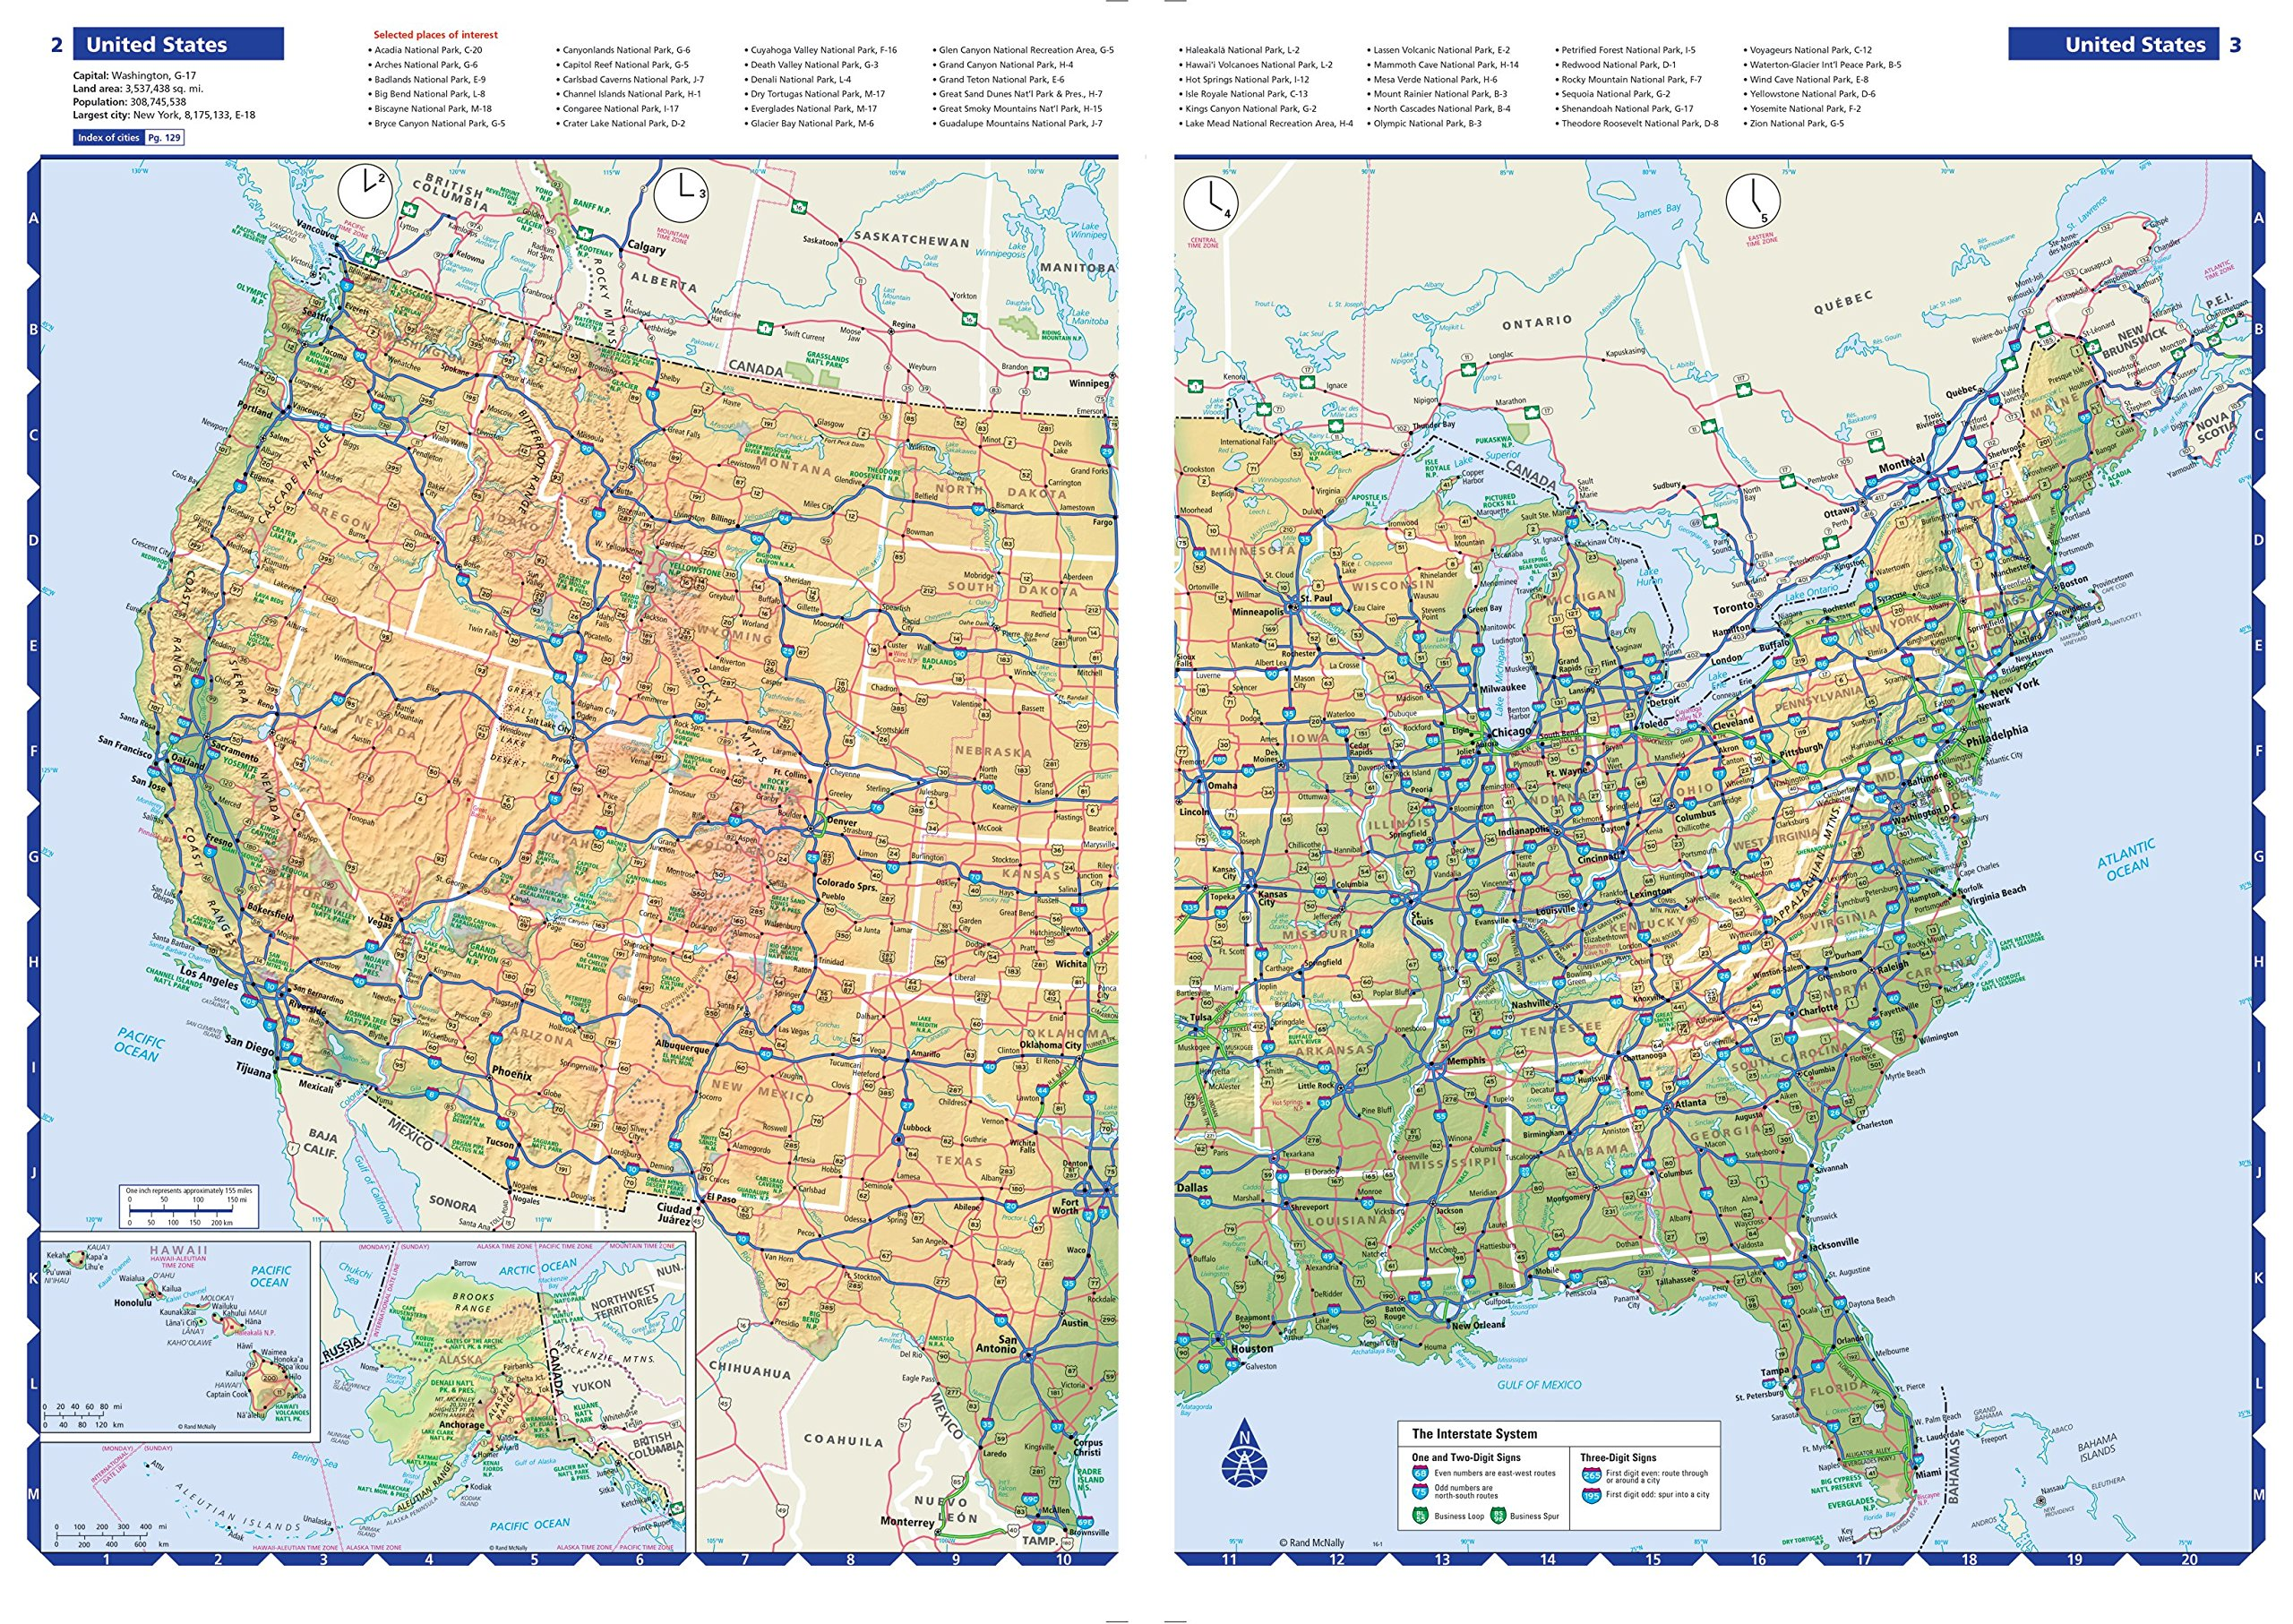
\includegraphics[scale=.1]{Semi_Riemannian/atlas.jpg}
        \end{frame}
    
        \begin{frame}{Smooth Manifold Structure}
            \begin{definition}
                A \textbf{smooth $m$-dimensional differentiable manifold} is a pair $(M,\mathcal{A})$ consisting of a \emph{(second countable) locally Euclidean space $M$ of dimension $m$} together with a \emph{differentiable structure $\mathcal{A}$}.
            \end{definition}
            \begin{remark}
                Second countable is a tool we want mathematically.  It's not farfetched physically. It just says each small patch on $M$ has a finite refinement.
            \end{remark}
        \end{frame}

        
        \begin{frame}{Smooth Manifold Structure}
            The picture to keep in your head:
            \begin{figure}
                \centering
                \includegraphics[scale=.75]{Riemannian_Geometry/smooth_manifold.png}
            \end{figure}
        \end{frame}
        
        
        \begin{frame}{Smooth Manifold Structure}
            \begin{textblock*}{6cm}(5cm,-2cm)
            \begin{itemize}
            \item[] \textbf{Summary}
                \item $M$ is the fundamental object, so charts map from $M$ to $\R^m$.
                \item $\psi \circ \varphi^{-1} \colon \varphi(U)\subset \R^m \to \R^m$,
                which means we can talk about derivatives.
                \item We require the transition map to be smooth on the overlap.
            \end{itemize}
            \end{textblock*}
            \begin{textblock*}{5cm}(0cm,-1.75cm)
            \includegraphics[scale=.55]{Semi_Riemannian/smooth_manifold.png}
            \end{textblock*}
        \end{frame}
        
        \begin{frame}{Examples of Smooth Manifolds}
            \begin{itemize}
                \item $\R^n$ (Lie Group)
                \item $S^n$ (Lie Group for some $n$)
                \item $T^n$ (Lie Group)
                \item \st{Simplicies}
                \item \st{$[0,1]^n$}
                \item $\mathrm{GL}_n(\R)$ (Lie Group)
                \item $\mathrm{SDiff}(M)$ (Infinite Dimensional Lie Group)
            \end{itemize}
        \end{frame}
        
        \begin{frame}{Notational Intervention}
            We usually refer to coordinates on a manifold in the following way: We know we have a chart $(U,\varphi)$ and that $\varphi(p)\in \R^m$.  We usually write:
            \[
            \varphi(p)=(x^1(p),\dots,x^m(p)).
            \]
            Each $x^i$ are commonly called coordinates as well.
        \end{frame}
        
        \begin{frame}{Smooth Manifold Structure}
            Questions? Thoughts?
        \end{frame}
        
        \begin{frame}{Functions}
            With the structure established, we next concern ourselves with functions (morphisms). Specific important functions:
            \begin{itemize}
                \item $f\colon M \to N$ with $M$ and $N$ smooth manifolds of $m$ and $n$-dimensions respectively. (Really, this is all of them.)
                \item $f\colon \R \to M$. Curves!
                \item $f\colon M \to \R$. 
            \end{itemize}
            What about isomorphisms?
            \begin{definition}
                A \textbf{diffeomorphism} is a smooth map $f\colon M \to N$ if $f$ is bijective with smooth inverse.
            \end{definition}
        \end{frame}
        
    \subsection{Fields}
        \begin{frame}{Functions}
        \begin{remark}
            What makes a map smooth? Think back to rubber sheets. In this case, we just cant make any sharp creases.
        \end{remark}
        We always work with coordinates! Let $(U,\varphi)$ and $(V,\psi)$ be coordinates on $M$ and $N$ respectively so that $f(U)\subset V$. Then:
        \begin{definition}
            A map $f\colon M\to N$ is \textbf{smooth} if 
            \[
            \hat{f}\coloneqq \psi \circ f \circ \varphi^{-1} \colon \varphi(U)\subset \R^m \to \psi(V)\subset \R^n,
            \]
            is smooth as a function from $\R^m \to \R^n$.
        \end{definition}
        \end{frame}
    
        \begin{frame}{Curves}
            \begin{textblock*}{6cm}(5cm,-2cm)
            \begin{itemize}
                \item Take a curve $\gamma \colon (-\epsilon,\epsilon)\to M$.
                \item Choose coordinates so $\gamma(0)=x\in M$.
                \item Consider 
                \[
                T_xM\ni v= \dot{\gamma}(0)\coloneqq \left.\frac{d}{dt}\gamma(t)\right|_{t=0}.
                \]
                \item Let $f\colon M \to \R$ be a smooth function.
                \item Then, we see how $\dot{\gamma}(0)$ acts on $f$.
            \end{itemize}
            \end{textblock*}
            \begin{textblock*}{5cm}(0cm,-1.75cm)
            \includegraphics[width=5cm]{Semi_Riemannian/tangent_space.png}
            \end{textblock*}
        \end{frame}
        
        \begin{frame}{Tangent Vectors}
            Note, we have $f\circ \gamma \colon (-\epsilon, \epsilon)\to \R$, which we can differentiate! Choose coordinates about $\gamma(0)$, $(U,\varphi)$. Then, let $\hat{\gamma}\coloneqq \varphi\circ \gamma$ so
            \[
            \hat{\gamma} \colon (-\epsilon,\epsilon) \to \R^m
            \]
            and denote
            \[
            \hat{\gamma}(t)=(x^1(t),\dots,x^m(t)).
            \]
            \begin{align*}
                \dot{\gamma}(0)(f)&\coloneqq \frac{d(f\circ \gamma)}{dt}(0)\\
                &=\left.\frac{d}{dt}\left( \underbrace{(f\circ \varphi^{-1})}_{\hat{f}}\circ \underbrace{(\varphi\circ \gamma)}_{\hat{\gamma}}\right)\right|_{t=0}\\
            \end{align*}
        \end{frame}
        
        \begin{frame}{Tangent Vectors}
        Keep going...
            \begin{align*}
                v&=\left.\frac{d}{dt}\left( \hat{f}(x^1(t),\dots,x^m(t))\right)\right|_{t=0}\\
                &=\sum_{i=1}^m \frac{\partial \hat{f}}{\partial x^i}(\hat{\gamma}(0))\frac{dx^i}{dt}(0)\\
                &=\left( \sum_{i=1}^m \dot{x}^i(0)\left( \frac{\partial}{\partial x^i}\right)_{\varphi(x)}\right)(\hat{f}).
            \end{align*}
        \end{frame}
        
        \begin{frame}{Tangent Vectors}
            \begin{paragraph}
                The previous work tells us that $\frac{\partial}{\partial x^i}$ form a basis for the \textbf{tangent space} (which always has dimension $m$) to $M$ at the point $x$ with the coordinates induced by $\varphi$. 
            \end{paragraph}
            \begin{remark}
                It was also the case that the coefficients for our basis vectors were $\dot{x}^i(0)$, the velocity components of the curve.
            \end{remark}
        \end{frame}
        
        \begin{frame}{Tangent Space and Bundle}
            \begin{textblock*}{6cm}(5cm,-2cm)
            \begin{itemize}
                \item Define the \textbf{tangent space to $M$ at the point $x$} (denoted $T_xM$) as the set of all tangent vectors to curves passing through the point $x$.
                \item Define the \textbf{tangent bundle of $M$} (denoted $TM$) as the union of all tangent spaces on $M$. (i.e., $TM=\bigcup_{x\in M}T_xM$.)
            \end{itemize}
            \end{textblock*}
            \begin{textblock*}{5cm}(0cm,-1.75cm)
            \includegraphics[width=5cm]{Riemannian_Geometry/tangent_space.png}
            \end{textblock*}
        \end{frame}


        \begin{frame}{Push Forwards}
            \begin{paragraph}
                Consider a smooth function $f\colon M \to N$.  Then, for a curve $\gamma$ on $M$, we can take $f\circ \gamma$ as a curve on $N$.  What is the tangent vector to $f\circ \gamma$ on $N$ at a point $x$?
            \end{paragraph}
        \end{frame}
        
        \begin{frame}{Push Forwards}
            \begin{paragraph}
                More generally, we want a diagram as follows:
            \end{paragraph}
            \[
            \begin{tikzcd}[ampersand replacement = \&, column sep=small]
            M \arrow[r, "f"] \& N \\
            TM \arrow[r, "f_*"'] \arrow[u, "\pi_M"] \& TN \arrow[u, "\pi_N"']
            \end{tikzcd}
            \]
            where $f_{*_x}$ is the unique linear map $T_xM \to T_{f(x)}N$.  In other words, $f_{*_x}=df_x$ is the \textbf{differential} of the function $f$. We call $f_*$ the \textbf{pushforward}.
            \begin{remark}
                Note the direction of the arrows. This transformation is covariant. This is to say, vector components are covariant.
            \end{remark}
        \end{frame}
        
        \begin{frame}{Push Forwards}
            \begin{example}
                Let $f\colon M \to N$ be smooth.  Then consider $(df)_p\colon T_pM \to T_{f(p)}N$.  If $v\in T_pM$ then $v=\dot{\gamma}(0)$ for some curve $\gamma$ and
                \[
                (df)_p(v)=\frac{d(f\circ \gamma)}{dt}(0).
                \]
                With basis $\frac{\partial}{\partial x^i}$ for $T_pM$ and $\frac{\partial}{\partial y^i}$ for $T_{f(p)}N$, we have
                \[
                (df)_p(v)=\sum_{i=1}^n\left( \sum_{k=1}^m v^k \left( \frac{\partial y^i}{\partial x^k}\right)(\varphi(0))\right)\left(\frac{\partial}{\partial y^i}\right)_{f(p)}.
                \]
            \end{example}
            \begin{remark}
                When working with coordinates, the differential is the jacobian (or the usual differential) you see in vector calculus.
            \end{remark}
        \end{frame}


        \begin{frame}{Cotangent Spaces}
            \begin{paragraph}
                With any vector space, we can consider the dual.  So we take $T_p^*M$ to be the dual to $T_pM$. What are the elements of $T_p^*M$?
            \end{paragraph}
            
            \vspace*{.5cm}
            
            \begin{paragraph}
                Consider $f\colon M \to \R$.  Then $(df)_p \colon T_pM \to T_{f(p)}\R\cong \R$.  This means $(df)_p \in T_p^*M$! 
            \end{paragraph}
            \vspace*{.5cm}
            \begin{paragraph}
                Well, what is $df_p$?
            \end{paragraph}
        \end{frame}

        \begin{frame}{Cotangent Spaces}
            Take $\gamma(t)=\varphi^{-1}(x^1(p)+v^1t,\dots,x^m(p)+v^m(t))$ so that $\dot{\gamma}(0)=v=v^i \frac{\partial}{\partial x^i}$ as a tangent vector in $T_pM$.
            \begin{align*}
                (df)_p(v)&\coloneqq v(f)=\left.\frac{d(f\circ \gamma)}{dt}\right|_{t=0}\\
                &= \left(v^i \frac{\partial \hat{f}}{\partial x^i}\right)(\varphi(p)),
            \end{align*}
            by the same computation as before. Then note that
            \begin{align*}
                (dx^i)_p(v)&=\frac{d(x^i\circ \gamma)}{dt}(0)\\
                &= \frac{d(x^i(p)+v^i t)}{dt}(0)\\
                &= v^i.
            \end{align*}
        \end{frame}
        
        \begin{frame}{Cotangent Spaces}
            Thus, it must be that
            \begin{align*}
                (df)_x &= \left(\frac{\partial \hat{f}}{\partial x^i}\right)(x(p))(dx^i)_x\\
                &=  \frac{\partial \hat{f}}{\partial x^1}(x(p))\left(dx^1\right)_x + ... + \frac{\partial \hat{f}}{\partial x^n}(x(p))\left(dx^n\right)_x.
            \end{align*}
            Moreover, the $dx^i$ form the canonical dual basis and we have
            \[
            dx^i\left( \frac{\partial}{\partial x^j}\right) = \frac{\partial}{\partial x^j}(x^i)=\delta_j^i.
            \]
        \end{frame}

        \begin{frame}{Cotangent Bundle}
            Just as before, we can define the \textbf{cotangent space of $M$ at the point $p$} (denoted $T_p^*M$) using the above $dx^i$ as the basis.  Then the \textbf{cotangent bundle of $M$} (denoted $T^*M$) is defined by $T^*M=\bigcup_{p\in M} T_p^*M$.) We refer to $dx^i$ as \textbf{one forms}.
        \end{frame}

        \begin{frame}{Pullbacks}
            In linear algebra, the dual linear transformation takes us the opposite direction.  Given a function $f\colon M \to N$, we have a diagram:
            \[
                \begin{tikzcd}[ampersand replacement=\&, column sep=small]
                M \arrow[r, "f"] \& N \\
                T^*M \arrow[u, "\pi_M"] \& T^*N \arrow[u, "\pi_N"'] \arrow[l, "f^*"]
                \end{tikzcd}            
            \]
            We call $f^*$ the \textbf{pullback} of $f$. 
            \begin{remark}
                Remember, forms pullback and vectors pushforward. Components of one forms behave in a contravariant way.
            \end{remark}
        \end{frame}
        
        \begin{frame}{Pullbacks}
        Recall:
        \[
                \begin{tikzcd}[ampersand replacement=\&, column sep=small]
                M \arrow[r, "f"] \& N \\
                T^*M \arrow[u, "\pi_M"] \& T^*N \arrow[u, "\pi_N"'] \arrow[l, "f^*"]
                \end{tikzcd}            
        \]
            \begin{example}
                Let $f\colon M \to N$ be smooth and $\omega \in T_{f(p)}^*N$.  Then, for $v\in T_pM$
                \begin{align*}
                    \underbrace{(f_p^* \omega)}_{\textrm{$T_p^*M$}}~~\underbrace{(v)}_{\textrm{$T_pM$}}=\underbrace{\omega}_{\textrm{$T_{f(p)}^*N$}}\underbrace{((df)_p(v))}_{\textrm{$T_{f(p)}N$}}.
                \end{align*}
            \end{example}
        \end{frame}
        
        \begin{frame}{Pause for a Moment}
            Questions? Thoughts?
        \end{frame}

        \begin{frame}{Tensors from a Physical Perspective}
            Tensors are \emph{exactly} measurements on a manifold. These are objects that remain invariant under changes of coordinates.  We require physical measurements to be independent of the choice of coordinates.
        \end{frame}
        
        \begin{frame}{(Tensor) Fields}
            A \textbf{$(p,q)$-tensor on $M$} is a smooth multilinear map
            \[
            \mathcal{T}\colon \underbrace{TM\times\cdots \times TM}_{p \textrm{~copies}}\times \underbrace{T^*M\times \cdots \times T^*M}_{q \textrm{~copies}} \to \R.
            \]
            It is in fact a \textbf{section} of a tensor bundle. 
            \begin{remark}
                $(0,0)$-tensors are \textbf{scalar fields}, $(0,1)$-tensors are \textbf{vector fields}, and $(1,0)$-tensors are \textbf{one forms}.
            \end{remark}
        \end{frame}
        
        \begin{frame}{Vector Fields}
            \begin{definition}
                A \textbf{vector field} on $M$ is a smooth map $X \colon M \to TM$ satisfying
                \[
                    \pi \circ X = \textrm{Id}_M.
                \]
                We usually denote the space of all vector fields by $\Gamma(TM).$
            \end{definition}
            \begin{remark}
                This requirement that $\pi \circ X = \textrm{Id}_M$ makes $X$ a \textbf{smooth section of the tangent bundle $TM$}.
            \end{remark}
            \begin{remark}
                A smooth vector field is an arrow at each point on a manifold so that these arrows vary smoothly.
            \end{remark}
        \end{frame}
        
        \begin{frame}{Fields}
            \begin{example}
                Consider $M=\R^2$. 
                \begin{itemize}
                    \item A scalar field $f\colon M \to R$ is given by $f(x_1,x_2)=x_1^2+x_2^2.$
                    \item A vector field is given by $X\colon M \to TM$ where $X_p = \left(\frac{\partial}{\partial x}\right)_p$.
                    \item A $(0,2)$-tensor field is given by $\mathcal{T}\colon M \to T^*M \otimes T^*M$ where $\mathcal{T}_p(X_p,Y_p)=\langle X_p, Y_p \rangle.$ Really, we have
                    \begin{align*}
                        \mathcal{T}_p(X_p,Y_p)&= \sum_{i,j=1}^m\delta_{ij}(dx^i \otimes dx^j)_p(X_p,Y_p)=\sum_{i=1}^m X_p^i Y_p^i.
                    \end{align*}
                    Which is exactly the Euclidean inner product! In physicists notation, we have $\mathcal{T}_p(X_p,Y_p)=\delta_{ij}X_p^iY_p^j.$
                \end{itemize}
            \end{example}
        \end{frame}

%%%%%%%%%%%%%%%%%%%%%%%%%%%%%%%%%%%%%%%%%%%%%%%%%%%%%%%%%%%%%%%%%%%%%%%%%%%%%%%
\section{Riemannian Geometry}
    \subsection{Metric Tensor Field}
	    \begin{frame}{$(0,2)$-Tensor Field}
            We define a map $G \colon TM \times TM \to \R$ by choosing coordinates and seeing how $G$ acts on vector fields at a point $p$ (i.e., $G(\cdot,\cdot)_p\colon T_pM\times T_pM \to \R$):
            \[
            G\left(X,Y \right)_p = (g_{ij})_p(dx^i \otimes dx^j)_p(X_p, Y_p).
            \]
            In other words, $G\colon M \to T^*M \otimes T^*M$, as before.
            \begin{remark}
                The metric is really captured by $g_{ij}$. In our previous example, $g_{ij}=\delta_{ij}$ was the flat (constant) Euclidean metric.
            \end{remark}
	    \end{frame}
	    
	    \begin{frame}{Riemannian Metric}
	        To build the Riemannian metric $(0,2)$-tensor field, we require
	        \begin{enumerate}[(i)]
	            \item \textbf{Symmetry:} $G(X,Y)_p=G(Y,X)_p$ for all $X,Y \in T_pM$.
	            \item \textbf{Nondegeneracy:} If $G(X,Y)_p=0$ for every $Y\in T_pM$, then $X_p\equiv 0$.
	            \item \textbf{Positive Definiteness:} $G(X,X)_p>0$ for all $X_p \in T_pM\setminus \{0\}$.
	        \end{enumerate}
	        We then get the coefficients $g_{ij}$ by noting how $G$ acts on basis vectors
	        \[
	        (g_{ij})_p\coloneqq G\left(\frac{\partial}{\partial x^i},\frac{\partial}{\partial x^j}\right)_p.
	        \]
	    \end{frame}
	    
	    \begin{frame}{Riemannian Manifolds}
	        \begin{question}
	        Are we asking too much to have a Riemannian metric?
	        \end{question}
	        \vspace*{0.5cm}
	        No! Not at all. Every smooth manifold admits a Riemannian metric. Let's take a step back and see why.
	    \end{frame}
	    
	    \begin{frame}{Embeddings}
	        \begin{definition}
	            Let $f\colon M \to N$ be smooth.  We call $f$ an \textbf{immersion} if $f_*$ is injective everywhere.  If $f$ is also a diffeomorphism onto its image, $f(M)$, then $f$ is a \textbf{embedding}.
	        \end{definition}
	        \begin{theorem}[Whitney]
	            Any smooth $m$-dimensional manifold can be embedded into $\R^{2m}$.
	        \end{theorem}
	    \end{frame}
	    
	
	    \begin{frame}{Musical Isomorphisms}
	        Recall the Riesz representation theorem which (roughly) says:
	        \begin{theorem}[Riesz]
	        If $V$ is an inner product space, then there is a canonical isomorphism from $V$ to $V^*$ given by
	        \begin{align*}
	        \flat \colon V &\to V^*\\
	        v &\mapsto v^\flat \coloneqq \langle v,\cdot \rangle.
	        \end{align*}
	        \end{theorem}
	    \end{frame}
	    
	    \begin{frame}{Musical Isomorphisms}
	        Similarly,
	        we have a map
	        \begin{align*}
	            \sharp \colon V^* &\to V\\
	            \omega &\mapsto \omega^\sharp,
	        \end{align*}
	        that we define by taking $\omega \in V^*$, $v\in V$, and setting
	        \[
	        \langle \omega^\sharp, v \rangle = \omega (v).
	        \]
	    \end{frame}
	    
	    \begin{frame}{Musical Isomorphisms}
	        We generalize this in the following way:
	        \begin{align*}
	            \flat \colon TM \to T^*M
	        \end{align*}
	        by
	        \[
	        (X^\flat)_p(Y)\coloneqq G(X,Y)_p \textrm{\quad Riesz, again}.
	        \]
	        And
	        \[
	            \sharp \colon T^*M \to TM
	        \]
	        by
	        \[
	        G(\omega^\sharp ,Y)_p = \omega_p(Y_p).
	        \]
	    \end{frame}
	    
	    \begin{frame}{Musical Isomorphisms}
	        \begin{example}
	            $\R^3$ has a very nice structure with these maps. We have the following
	            \begin{figure}[htbp]
                \begin{tikzpicture}[node distance=2cm, auto]
	            \node (O0) {$\Omega^0(M)$};
	            \node (O1) [right of=O0] {$\Omega^1(M)$};
	            \node (O2) [right of=O1] {$\Omega^2(M)$};
	            \node (O3) [right of=O2] {$\Omega^3(M)$};
	            \node (F1) [below of=O0] {$C^\infty(M)$};
	            \node (V1) [below of=O1] {$\mathfrak{X}(M)$};
	            \node (V2) [below of=O2] {$\mathfrak{X}(M)$};
	            \node (F2) [below of=O3] {$C^\infty(M)$};
	            \draw[->] (O0) to node {$d$} (O1);
	            \draw[->] (O1) to node {$d$} (O2);
	            \draw[->] (O2) to node {$d$} (O3);
	            \draw[->] (F1) to node {$\nabla$} (V1);
	            \draw[->] (V1) to node {$\nabla \times$} (V2);
	            \draw[->] (V2) to node {$\nabla \cdot$} (F2);
	            \draw[->] (F1) to node {$\mathrm{id}$} (O0);
	            \draw[->] (V1) to node {$\flat$} (O1);
	            \draw[->] (V2) to node {$\star^\flat$} (O2);
	            \draw[->] (F2) to node [swap] {$\star$} (O3);
            \end{tikzpicture}
            \label{fig:diagram}
            \end{figure}
            This takes a bit more time to unravel, but the connection between forms and vectors here is key. We require a metric for this!
	        \end{example}
	    \end{frame}

        \begin{frame}{Distance Function}
            \begin{question}
            How is the metric actually a metric?
            \end{question}
            \vspace*{0.5cm}
            Well, it extends to a length function on curves!
        \end{frame}
        
        \begin{frame}{Distance Function}
            \begin{question}
                How do we compute distances physically? 
            \end{question}
            \vspace*{0.5cm}
            We must know the total time and speed.  In our case
            \begin{definition}
                The \textbf{speed of a curve $\gamma$ at time $t$} is given by
                \[
                \|\dot{\gamma}(t)\|\coloneqq \sqrt{G(\dot{\gamma}(t),\dot{\gamma}(t))_{\gamma(t)}}.
                \]
            \end{definition}
        \end{frame}
        
        \begin{frame}{Distance Function}
            Now, taking this, we can just integrate over whatever time period we care to. Take $\gamma \colon [t_0,t_1] \to M$, then
            \[
            l(\gamma)\coloneqq \int_{t_0}^{t_1} \|\dot{\gamma}(t)\|dt.
            \]
            \begin{remark}
            This is almost an equation for energy.  Remember, $E=\frac{1}{2}mv^2$.  We can also write
            \[
            E(\gamma)\coloneqq \frac{1}{2}\int_{t_0}^{t_1}G(\dot{\gamma}(t),\dot{\gamma}(t))_{\gamma(t)}dt.
            \]
            \end{remark}
        \end{frame}
        
        \begin{frame}{Distance Function}
            Now, we define the \textbf{distance} as follows:
            \begin{definition}
                Let $p,q\in M$, then
                \[
                \textrm{d}(p,q)\coloneqq \inf \{l(\gamma)~\vert~\gamma \colon [0,1] \to M, ~\gamma(0)=p,~\gamma(1)=q \}
                \]
            \end{definition}
            \vspace*{0.5cm}
            When this infumum exists, it is realized by a curve $\gamma$ called an \textbf{geodesic}.
        \end{frame}

	
    \subsection{Examples}
    
        \begin{frame}{Embeddings into $\R^n$}
            Whitney said we can embed $M$ into $\R^n$ by some $f$ and our pushforward is injective.  $\R^n$ already has a canonical metric (the flat metric), which we can pullback onto $M$ by
            \[
            (f^* g^{\R^n})(v,w)=g^{\R^n}(df(v),df(w)).
            \]
            \begin{remark}
                The moral of the story here is that you can picture $M$ sitting in $\R^n$, and this visual gives you all the properties on $M$ you could want.
            \end{remark}
        \end{frame}
        
        \begin{frame}{Working With $S^2$}
            Let us work through all of this with an explicit example.
            \vspace*{0.5cm}
            Let $S^2 = \{x \in \R^3 ~\vert~ \|x\|=1\}$. We want to show $S^2$ is a smooth manifold, find the tangent spaces, and construct a metric. 
        \end{frame}
        
        \begin{frame}{Working With $S^2$}
                To see $S^2$ is a smooth manifold, we take two charts $(\mathcal{N},\pi_\mathcal{N})$ and $(\mathcal{S},\pi_\mathcal{S})$ where $\mathcal{N}$ is the open set containing all points but the south pole, and $\mathcal{S}$ is the open set containing all points but the north pole.
                
                Now, define 
                \[
                \pi_{\mathcal{N}}\underbrace{(x_1,x_2,x_3)}_{\textrm{on $S^2 \subset \R^3$}}=\left(\frac{x_1}{1-x_3},\frac{x_2}{1-x_3}\right),
                \]
                which has inverse
                \[
                \pi_{\mathcal{N}}^{-1}\underbrace{(X_1,X_2)}_{\textrm{in $\R^2$}}=\left(\frac{2X_1}{1+X_1^2+X_2^2},\frac{2X_2}{1+X_1^2+X_2^2},\frac{-1+X_1^2+X_2^2}{1+X_1^2+X_2^2}\right).
                \]
        \end{frame}
        
        \begin{frame}{Working With $S^2$}
                Here is a picture of what we did:
                \begin{figure}
                    \centering
                    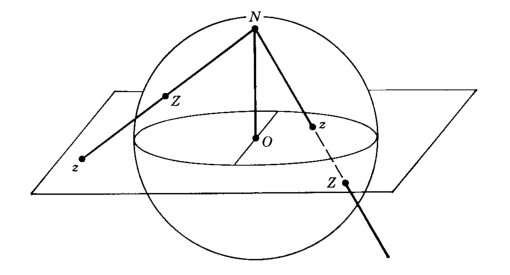
\includegraphics[scale=0.35]{Semi_Riemannian/stereographic.jpg}
                \end{figure}
        \end{frame}
        
        \begin{frame}{Working With $S^2$}
            The chart $(\mathcal{S},\pi_\mathcal{S})$ is very analogous.
            \vspace*{0.5cm}
            \begin{question}
                What else must we show?
            \end{question}
        \end{frame}
        
        \begin{frame}{Working With $S^2$}
            \begin{question}
                Are the transition functions $\pi_{\mathcal{S}}\circ \pi_{\mathcal{N}}^{-1}$ and $\pi_{\mathcal{N}}\circ \pi_{\mathcal{S}}^{-1}$ both smooth?
            \end{question}
            \vspace*{0.5cm}
            Yes, in fact
            \[
            \pi_\mathcal{N}\circ \pi_\mathcal{S}^{-1} = \pi_\mathcal{S} \circ \pi_\mathcal{N}^{-1}(p)=\frac{1}{\|p\|}p,
            \]
            which is defined everywhere except $p=0$, which is either the north or south pole.  The transition is smooth. Since our two charts cover $S^2$, we've shown $S^2$ is a smooth manifold.
        \end{frame}
        
        \begin{frame}{Working With $S^2$}
            We can compute the tangent space at the north pole $(0,0,1)$, by letting $\gamma \colon (-\epsilon, \epsilon) \to S^2$ be defined by
            \[
            \gamma(t)=(t\cos \theta, t\sin \theta, \sqrt{1-t^2}).
            \]
            We can choose a chart $(U,\varphi)$ on $S^2$ which takes the northern hemisphere and projects it into the $xy$-plane. 
            \[
            \varphi(x,y,z)=(x,y)
            \]
            and
            \[
            \varphi^{-1}(X,Y)=(X,Y,\sqrt{1-X^2-Y^2}).
            \]
        \end{frame}
        
        \begin{frame}{Working With $S^2$}
            Now, for some $f\colon S^2 \to \R$, we take
            \begin{align*}
                \dot{\gamma}(0)(\hat{f})&=\left. \frac{d}{dt}((\hat{f}(t\cos \theta, t \sin \theta))\right|_{t=0}\\
                &= \left.\left(\frac{\partial \hat{f}}{\partial x} \frac{d}{dt}(t\cos \theta) + \frac{\partial \hat{f}}{\partial y}\frac{d}{dt} (t \sin \theta)\right)\right|_{t=0}\\
                &= \left( \cos \theta \frac{\partial}{\partial x}+\sin \theta \frac{\partial}{\partial y}\right)(\hat{f})(0).
            \end{align*}
            For a choice of $\theta$, we've found a (unit) vector in the tangent space at the north pole.  You can repeat this process at any point on $S^2$.
        \end{frame}
        
        \begin{frame}{Working With $S^2$}
            By noting we have an embedding $S^2\subset \R^3$, we can look at the pullback metric (also called the induced metric). Take $(\varphi,U)$ be a chart on the northern hemisphere given by
            \[
            \varphi(x^1,x^2)=\left(x^1,x^2,\sqrt{1-(x^1)^2-(x^2)}\right)
            \]
            (Based on previous notation, this should be $\varphi^{-1}$.)
        \end{frame}
        
        \begin{frame}{Working With $S^2$}
            We then look at $g\coloneqq \varphi^* \delta$ ($\delta$ the usual metric on $\R^3$) which is given by
            \[
            g_{ij}=(\varphi^* \delta)_{ij} = \varphi^*\left\langle \frac{\partial}{\partial x^i}, \frac{\partial}{\partial x^j}\right\rangle =\left\langle \frac{\partial \varphi}{\partial x^i}, \frac{\partial \varphi}{\partial x^j}\right\rangle.
            \]
            We then get
            \[
            g_{ij}=\delta_{ij} + \frac{x^i x^j}{1-(x^1)^2-(x^2)^2}.
            \]
            We call $S^2$ with this metric $g$ the \textbf{round sphere}.
        \end{frame}
        
        \begin{frame}[End]
            Questions? More examples?
        \end{frame}

\end{document}